\documentclass[a4paper,12pt]{article}
\usepackage{HomeWorkTemplate}
\usepackage{circuitikz}
\usepackage[shortlabels]{enumitem}
\usepackage{hyperref}
\usepackage{tikz}
\usepackage{amsmath}
\usepackage{amssymb}
\usepackage{tcolorbox}
\usepackage{xepersian}
\usepackage{mathtools}
\settextfont{XB Niloofar}
\usetikzlibrary{arrows,automata}
\usetikzlibrary{circuits.logic.US}
\usepackage{changepage}
\newcounter{subproblemcounter}
\setcounter{subproblemcounter}{1}
\newcommand{\problem}[1]
{
	\subsection*{
		تمرین
		#1
		}
	\setcounter{subproblemcounter}{1}
}
\newcommand{\subproblem}{
	\textbf{\harfi{subproblemcounter})}\stepcounter{subproblemcounter}
}


\begin{document}
\handout
{مباحث ویژه در سیستم‌های دیجیتال}
{دکتر ایمان غلام‌پور}
{نیم‌سال اول 1400\lr{-}1401}
{اطلاعیه}
{امین کشیری}
{۹۷۱۰۱۰۲۶}
 {تمرین سری چهارم}

\problem{۱}
\

\subproblem
اگر هر 
k
سطری که انتخاب می‌کنیم،‌ مقدار ۰ داشته باشند، نتیجه‌ی 
minHash
برابر با 
\lr{don't know}
 می‌شود زیرا مکان اولین ۱ را نمی‌توان پیدا کرد. برای این که این اتفاق رخ دهد، باید احتمال این که 
 k 
 سطر انتخاب کنیم و همه برابر با ۱ باشند را به دست آوریم. این احتمال برابر است با :
 \begin{LTR}
 $P = (\frac{n-m}{n}) \times (\frac{n-m-1}{n-1}) \cdots (\frac{n-m-k+1}{n-k+1}) \approx (\frac{n-m}{n})^k$
 \end{LTR}
 که در واقع هر کسر از تقسیم تعداد صفر‌های باقی مانده به تعداد کل درایه‌ها به دست می‌آید. 


 \subproblem
 می‌خواهیم: 
 \begin{LTR}
 $ (\frac{n-m}{n})^k \leq e^{-10} \Rightarrow  (1 - \frac{1}{\frac{n}{m}})^{\frac{n}{m}\frac{mk}{n}} \leq e^{-10} \xrightarrow{m \ll n} e^{\frac{-mk}{n}} \leq e^{-10} \rightarrow -\frac{mk}{n} \leq -10$
 
 $ \rightarrow k \geq \frac{10n}{m}$
 \end{LTR}

پس کوچک‌ترین مقدار 
k
که احتمال وقوع 
\lr{don't know}
برابر با مقدار داده‌شده شود برابر است با 
$\frac{10n}{m}$.


\problem{۲}
\ 

\subproblem
FP
وقتی رخ می‌دهد که به اشتباه دو اثر انگشت که با هم شبیه نیستند را شبیه تشخیص دهیم. احتمال این که چنین اتفاقی بیفتد (با یک هش)، برابر است با احتمال این که ۶ خانه 
به صورت تصادفی، 
minutiae
 داشته باشند، که این احتمال برابر است با 
$p_{FP} = (0.2)^6 = 0.000064$. 
حال اگر دو اثر انگشت یکسان باشند، احتمال این که در ۳ خانه‌ی یک تابع هش خاص، 
minutiae
 وجود داشته باشد برابر است با 
 $(0.2)^3$.
 در این صورت احتمال این که تصویر دیگری از همان اثر انگشت هم همین خاصیت را داشته باشد برابر است با 
 $(0.8)^3$. 
 پس احتمال شبیه تشخیص دادن این ۲ برابر است با ضرب این دو احتمال و احتمال رخ دادن 
 FN
 برابر است با :
 $p_{FN} = 1 - (0.2)^3 \cdot (0.8)^3 = 0.9959$. 
 حال اگر از ۱۰۲۴ تابع هش استفاده کنیم و با هم 
 OR
  کنیم، احتمال این که به اشتباه یکی از هش‌ها یکی شود برابر است با:
  \begin{LTR}
	$P_{FP} = 1 - (1-p_{FP})^{2048} =0.1228$
  \end{LTR}
  که احتمال 
  FP
  است. همچنین، احتمال این که هیچ‌کدام از هش‌ها برای دو اثر انگشت یکسان یکی نشود، برابر است با :
  \begin{LTR}
  $P_{FN} = (p_{FN})^{2048} = 0.0002236$                                                       
  \end{LTR}
 که همان احتمال 
 FN  
 است. 
 در حالت دوم، که توابع هش را به دو گروه تقسیم می‌کنیم، باید ترکیبی از این دو حالت را در نظر بگیریم. 
 احتمال رخ دادن 
 FP
 برابر است با این که در هر دو دسته 
 FP
 رخ دهد. پس:
\begin{LTR}
	$P_{FP} = (P_1)_{FP} \times (P_2)_{FP} = (1 - (1-p_{FP})^{1024})^2 = 0.004 $
\end{LTR}
از طرفی برای رخ دادن
FN
کافی است یک از دو دسته 
FN
شود. در این صورت داریم:
\begin{LTR}
$P_{FN} = 1 - (1-(P_2)_{FN}) \times (1-(P_2)_{FN}) = 1 - (1-(p_{FN})^{1024})^2 = 0.02968$
\end{LTR}


\subproblem
فرمول‌های به دست آمده برای هر دو حالت را بر حسب 
n
می‌نویسیم. در حالت اول داشتیم:
\begin{LTR}
	$P_{FP} = 1 - (1-p_{FP})^{n}$
	
	$P_{FN} = (p_{FN})^{n}$       
	
	$P_t = 1 - (1-p_{FP})^{n} +  (p_{FN})^{n}$       
\end{LTR}
اما در حالت دوم داریم: 
\begin{LTR}
	$P_{FP} = (P_1)_{FP} \times (P_2)_{FP} = (1 - (1-p_{FP})^{\frac{n}{2}})^2 $
	
	$P_{FN} = 1 - (1-(P_2)_{FN}) \times (1-(P_2)_{FN}) = 1 - (1-(p_{FN})^{\frac{n}{2}})^2 $

	$P_t = (1 - (1-p_{FP})^{\frac{n}{2}})^2  + 1 - (1-(p_{FN})^{\frac{n}{2}})^2 $
\end{LTR}

حال کافی است از
$P_t$
بر حسب 
n 
مشتق بگیریم. در حالت اول:
\begin{LTR}
	$\frac{\partial P_t}{n} = - \ln (1-p_{FP})(1-p_{FP})^n + \ln(p_{FN})(p_{FN})^n = 0$

	$\frac{\ln(p_{FN})}{\ln({1-p_{FP}})} = (\frac{1-p_{FP}}{p_{FN}})^n \Rightarrow 
	\ln(\frac{\ln(p_{FN})}{\ln({1-p_{FP}})} ) / \ln(\frac{1-p_{FP}}{p_{FN}}) = n$
\end{LTR}

که با توجه به مقادیر 
$p_{FP}$
و
$p_{FN}$
داریم: 
\begin{LTR}
$n \approxeq 1029$
\end{LTR}
 
در حالت دوم، به صورت مشابه جلو می‌رویم. با مشتق گرفتن و برابر صفر قراردادن و جایگذاری احتمال‌ها داریم (شکل جواب بر حسب 
n
مانند شکل زیر است):
\begin{LTR}
$n \approxeq 3210$
\end{LTR}

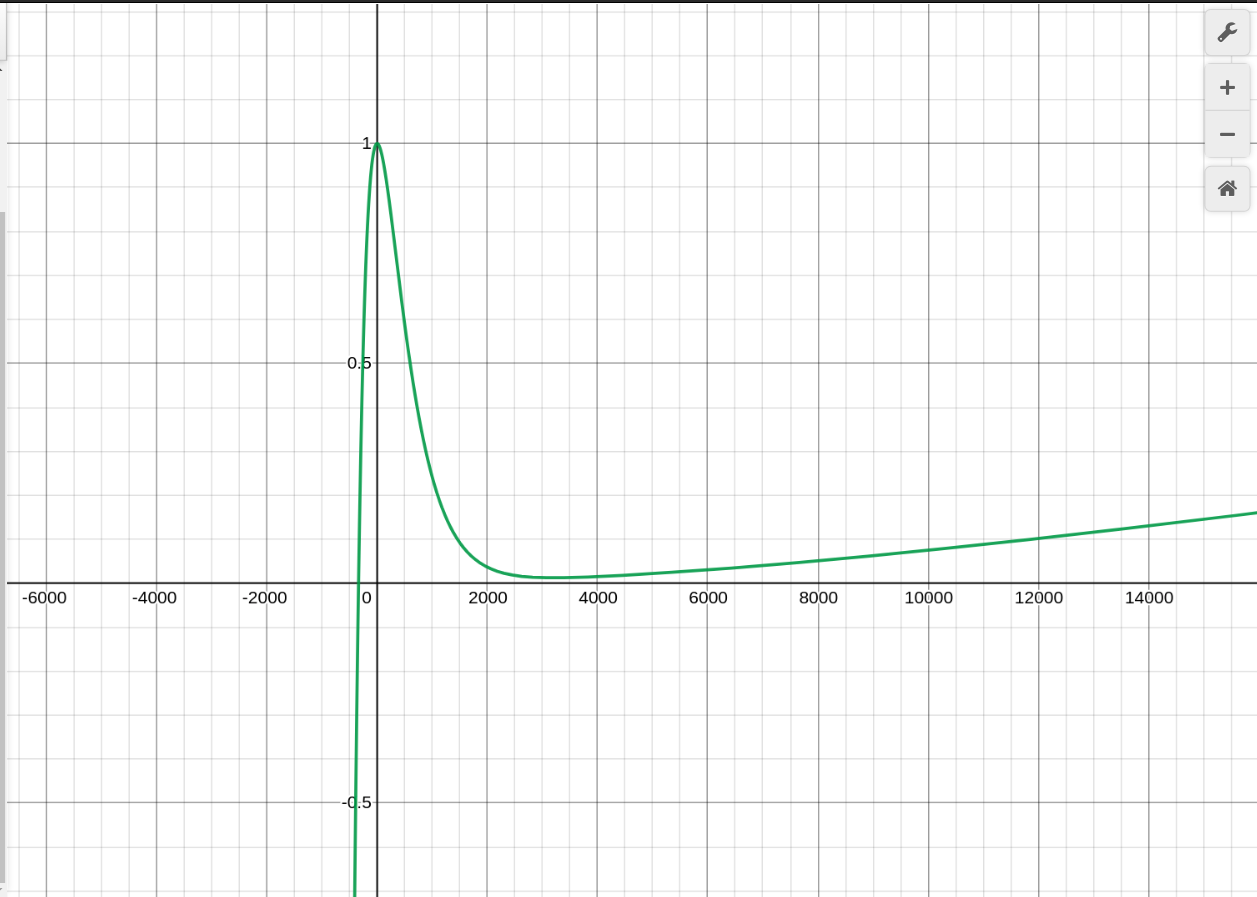
\includegraphics[scale=0.4]{p2.png}




\problem{۴}
\ 

ابتدا مراحل این الگوریتم را بررسی می‌کنیم. تعریف‌هایی که در این متن می‌بینید با تعریف‌های کتاب هماهنگ هستند. 

مهم است که بدانیم هر کلاستر را در این الگوریتم چگونه نمایش بدهیم. دقت کنید که نگه داشتن تمامی نقاط یک کلاستر ممکن است به دلیل حجم بالا و حجم پایین حافظه‌ی اصلی ممکن 
نباشد. برای هر نقطه در هر کلاستر
ROWSUM
این نقطه را تعریف می‌کنیم مجموع مجذور فاصله‌ی این نقطه تا تمامی نقاط دیگر این کلاستر. حال به عنوان نماینده‌ی یک کلاستر، اطلاعت زیر را نگه می‌داریم: 

\begin{enumerate}
	\item 
	N
	که همان تعداد نقاط کلاستر است. 

	\item 
	مرکز 
	(clustroid)
	یک کلاستر، که نقطه‌ای از کلاستر تعریف می‌شود که 
	ROWSUM 
	آن کمینه است. 

	\item 
	ROWSUM
	مرکز کلاستر. 

	\item 
	k
	نقطه‌ای که بیش از همه به مرکز نزدیک‌اند، که 
	k
	عددی انتخابی است. 

	\item 
	k
	نقطه‌ای که بیش از همه از مرکز دورند (اما عضو کلاستر هستند).
\end{enumerate}

\textbf{درخت کلاستر}

کلاستر‌ها را به کمک درخت‌هایی (مانند
\lr{B-Tree}ها) 
نگه می‌داریم. برگ‌های درخت، تا جایی که می‌توانند نماینده‌ کلاستر‌ها را نگه 
می‌دارند. گره‌های میانی، نمونه‌ای از مرکز کلاستر‌هایی که در زیردرختش 
قرار دارند را نگه می‌دارد، به علاوه‌ی نشانه‌ی به برگی که نماینده این کلاستر را در خود نگه داشته است.
برای شروع الگوریتم نیاز داریم که سمپلی که در 
حافظه‌ی اصلی داریم را به صورت
hierarchial
کلاستر کنیم. اما دقت کنید که این درخت نهایی نیست و باید به کمک آن 
درخت اصلی الگوریتم خود را بسازیم. 




\textbf{مراحل بعدی الگوریتم}

هر نقطه‌ای که می‌خواهیم به کلاسترهای خود اضافه کنیم، را ابتدا با ریشه‌ی درخت 
مقایسه می‌کنیم. نزدیک ترین مرکزی که نگه داشته‌ایم را پیدا می‌کنیم و 
با کمک نشانه‌ی زیر درختش، یک مرحله از درخت پایین می‌رویم. این مراحل را آنقدر 
ادامه می‌دهیم تا به یک برگ برسیم. حال این نقطه را به کلاستر نزدیک ترین مرکز 
نگه داشته شده اضافه می‌کنیم. با این کار، نماینده‌ی آن کلاستر به کلی تغیر می‌کند. در این مرحله مرکز کلاستر 
جدید را تغییر نمی‌دهیم اما 
ROWSUM
نقطه‌ی اضافه شده را تخمین می‌زنیم. 


هرگاه شعاع یک کلاستر از حدی (که الگوریتم تعیین می‌کند) بزرگتر شد، باید آن را 
به دو کلاستر مجزا تقسیم کنیم. این کار را به گونه‌ای انجام می‌دهیم که 
ROWSUM
دو مرکز جدید کمینه شود. دقت کنید که شعاع کلاستر‌ها را به کمک
k
تا دورترین نقطه‌ی کلاستر می‌توانیم به دست آوریم. در این مراحل، باید ساختار 
\lr{B-Tree}
خود را حفظ کنیم،‌که الگوریتم‌ خاص خود را دارند. 
اگر تعداد کلاستر‌های ما زیاد شوند، و دیگر اطلاعت آن‌ها به سختی در حافظه جا بگیرد، ما مجبور به 
ترکیب کردن دو کلاستر می‌شویم. برای پیدا کردن مرکز جدید، به کمک دورترین نقاط هر کلاستر، مرکز جدید 
را به دست می‌آوریم. این مراحل را آنقدر ادامه می‌دهیم که کلاستر‌های نهایی را به دست آوریم. 



\textbf{کاربرد‌های الگوریتم}

الگوریتم
GRGPF
در زمان‌هایی به کار می‌رود که داده‌ی ما بسیار زیاد باشد. دقت کنید که این الگوریتم نیازی به نگه داشتن 
تمامی داده‌ها در حافظهی اصلی ندارد، و این مزیت بزرگی محسوب می‌شود. یک نکته‌ی مثبت دیگر این الگوریتم این است که 
نیازی به فضای اقلیدسی ندارد. بنابرین در مکان‌هایی که اشکال تشکیل کلاستر‌های ما شکل متقارنی ندارند نیز می‌تواند به کار گرفته شود. همچنین، در کاربردهایی 
که فضای اقلیدسی برای مسائل امکان پذیر نیست (ابعاد بسیار بالا) این الگوریتم می‌تواند بدون درگیر شدن با 
نفرین ابعاد بزرگ (به دلیل دوری از فضای اقلیدسی) مسئله را برای ما حل کند. 
\end{document}